\documentclass{beamer}

\title{Searching for Hidden Objects}
\subtitle{Looking for custard cups in mixing bowls, and not the other way around}
\author{Troy Astorino, Neil Forrester}
\date{April 10, 2013}
\institute[6.834 -- MIT]{Cognitive Robotics \\ Massachusetts Institute of Technology}

\usepackage{graphicx}
\usepackage{amsmath}

\usetheme{CambridgeUS}
\usecolortheme{beaver}
\setbeamertemplate{section in toc}[square]
%\setbeamercolor{section number projected}[bg=black, fg=red]
\setbeamertemplate{navigation symbols}{} % remove navigation symbols

% \argmax operator
\DeclareMathOperator*{\argmax}{arg\,max}

% \norm{n}{stuff} is the L-n norm of stuff
\providecommand{\norm}[2]{\lVert#2\rVert_#1}

\newcommand{\overlay}[3]{\includegraphics<#3>[scale=#2]{img/#1.png}}
\newcommand{\overlayL}[2]{\overlay{#1}{0.5}{#2}}
\newcommand{\overlayM}[2]{\overlay{#1}{0.3}{#2}}

% macros for including shape pictures at various scales (Large, Medium, Small)
\def \spL [#1]{\overlayL{#1}{1}}
\def \spM [#1]{\overlayM{#1}{1}}
\def \spS [#1]{\overlay{#1}{0.15}{1}}

% uncomment this with your current latex file to only compile it
%\includeonly{mcmc}
\begin{document}

\section{Introduction}
\section{section title}
\begin{frame}
  \frametitle{The necessity of manipulation-based search}
  \begin{center}
    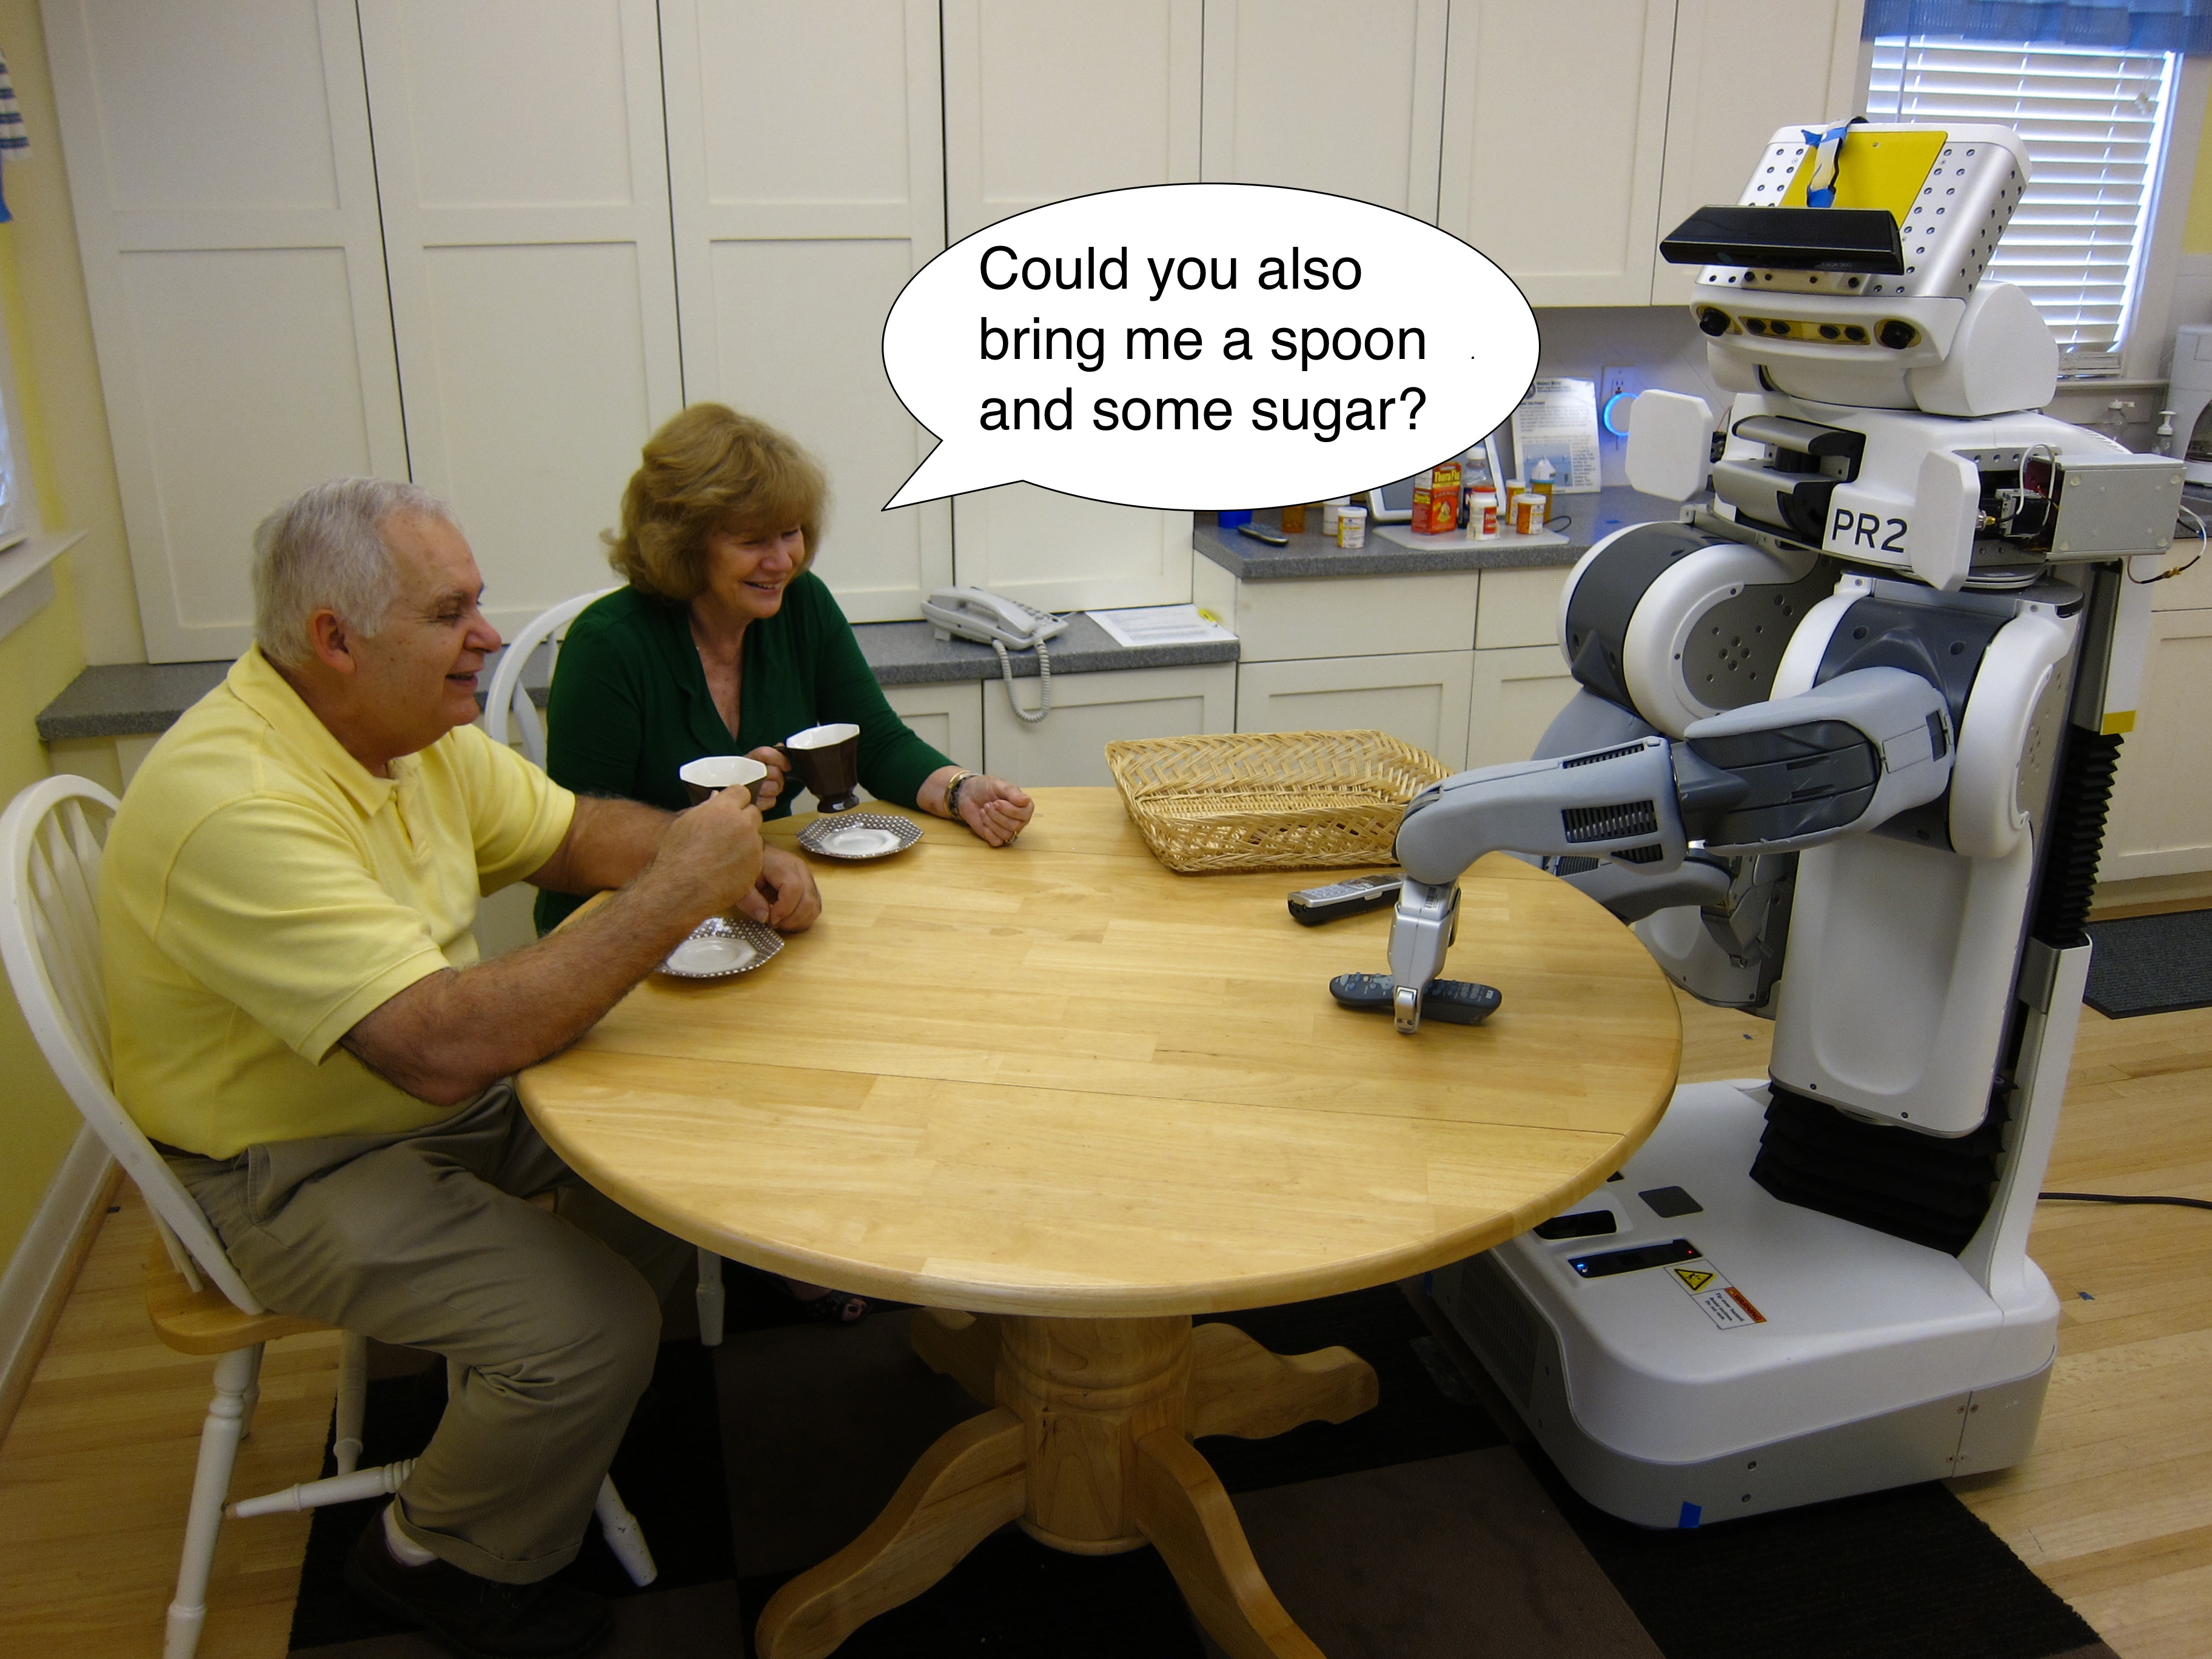
\includegraphics[width=3.2in]{img/robot_in_kitchen.jpg}

    \tiny{Original image courtesy of Wendy Rogers/Georgia Tech}
  \end{center}
\end{frame}

\begin{frame}
  \frametitle{The necessity of manipulation-based search}
  \begin{center}
    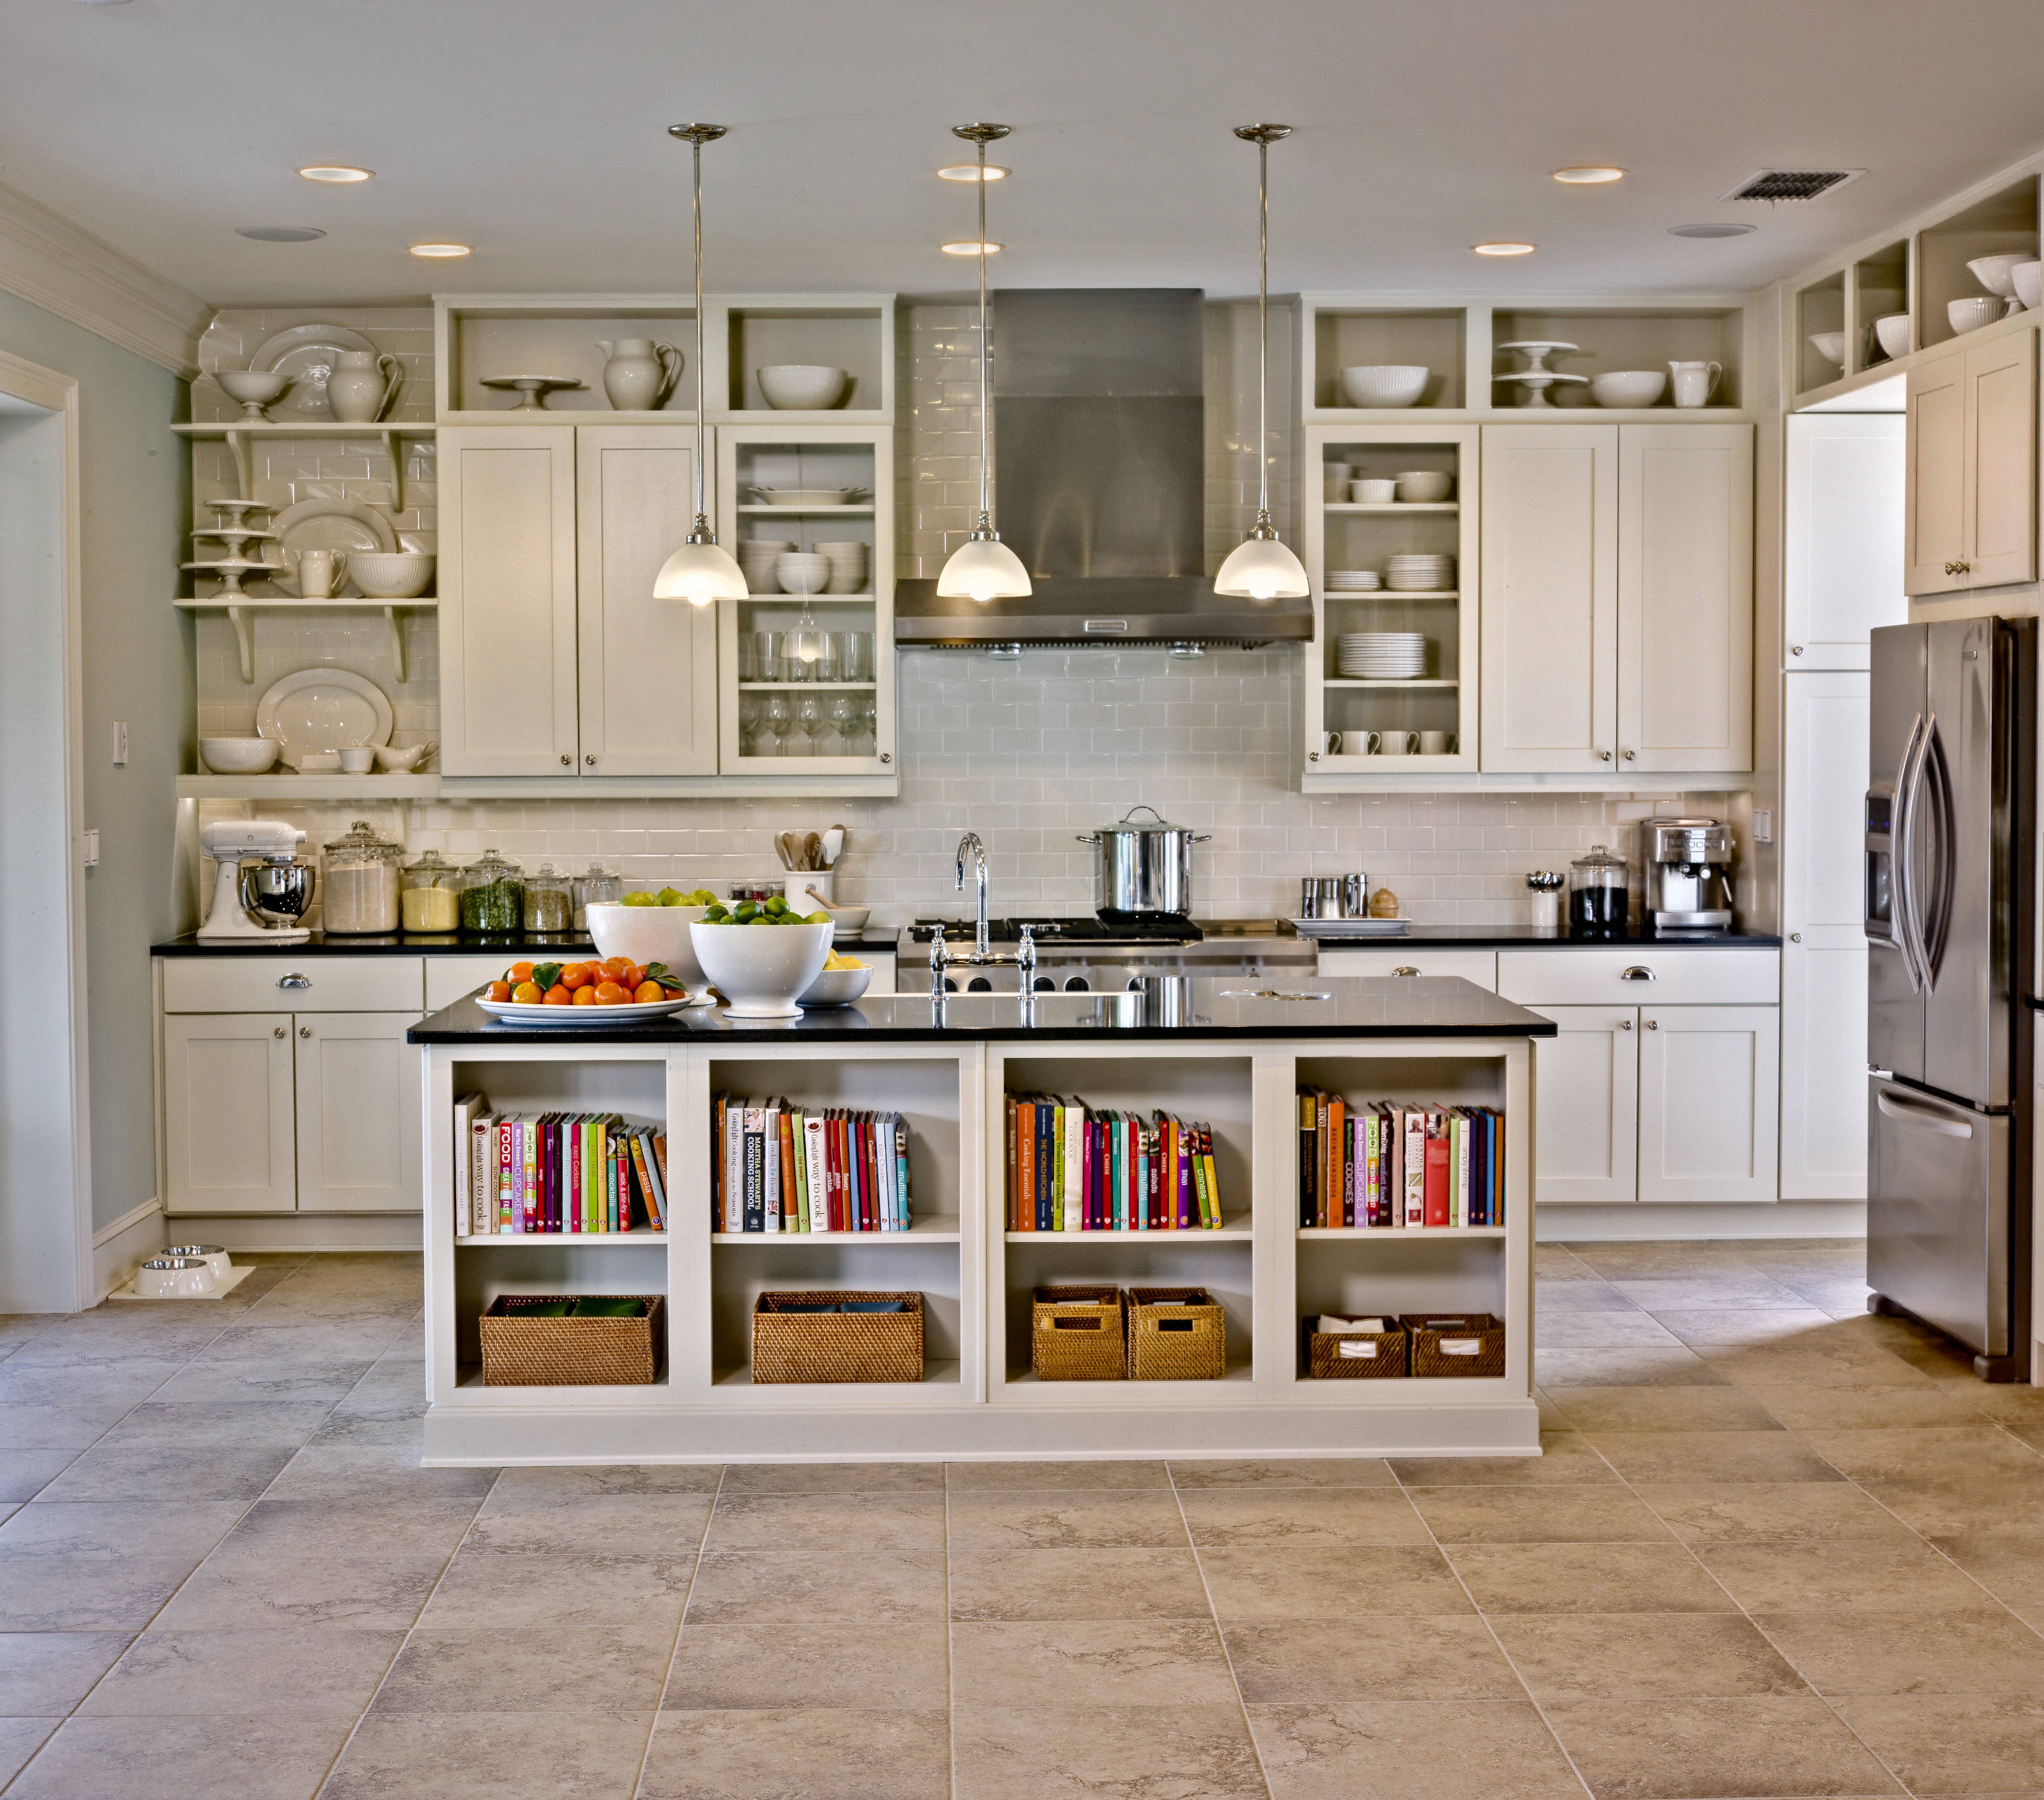
\includegraphics[height=2.7in]{img/kitchen-organization-fake.jpg}

    \tiny{Original image courtesy of personalorganizing.about.com}
  \end{center}
\end{frame}

\begin{frame}
  \frametitle{The necessity of manipulation-based search}
  \vspace{-0.3in}
  \begin{columns}
    \begin{column}{0.6\textwidth}
      \begin{itemize}
        \item Some things are hidden behind other things.
        \item We have to remove items in front to see items in back.
        \item The cookie tray and the rat poison are not likely to be on the same shelf.
      \end{itemize}
    \end{column}
    \begin{column}{0.4\textwidth}
      \begin{center}
        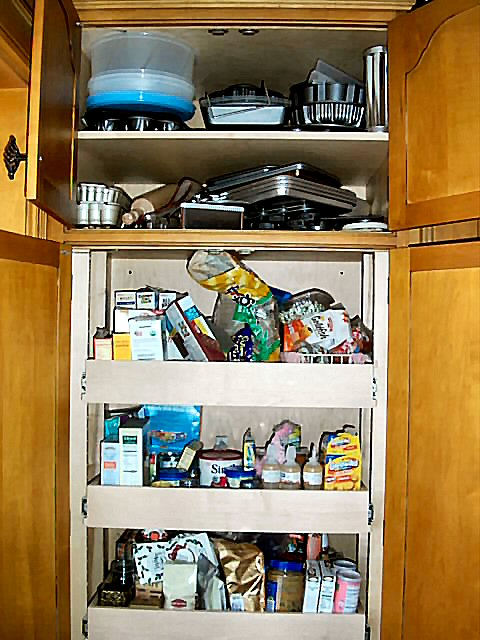
\includegraphics[height=2.7in]{img/kitchen-organization.jpg}

        \tiny{Original image courtesy of shilloh.com}
      \end{center}
    \end{column}
  \end{columns}
\end{frame}

\begin{frame}
  \frametitle{Assumptions for the following treatment}
  \begin{itemize}
  \item No errors in  visual identification and classification of objects
  \item Robot can successfully complete any movement and manipulation task, but
    these are temporally expensive
  \item Finite set of object types in the world
  \end{itemize}
\end{frame}


\section{Probability Distributions in Robotics}
\begin{frame}
  \frametitle{Dichlet distribution}
\end{frame}

\begin{frame}
  \frametitle{Gaussian distribution}
\end{frame}

\begin{frame}
  \frametitle{Logistic transformations}
\end{frame}


\section{Maximum Likelihood Estimation}
\begin{frame}
  
\end{frame}

\section{Markov chain Monte Carlo}
\begin{frame}
  \frametitle{Markov chain Monte Carlo}
  Allows sampling from a probability distribution whose form is not explicitly
  known.
\end{frame}

\begin{frame}
  \frametitle{Metropolis-Hastings Algorithm}
  \begin{center}
    Draws samples from any probability distribution $P(x)$, as long as a
    function $f(x)$ proportional to the probability distribution is known
    \vspace{4em}

    Very useful in Bayesian inference for non-conjugate posteriors in
    multi-dimensional vector spaces
    \[P(x|h) \propto P(h|x) P(x)\]
  \end{center}
\end{frame}

\begin{frame}
  \frametitle{Overview of Algorithm}
  \begin{itemize}
  \item Draws samples from $P(x)$ by taking a type of random walk about $f(x)$
  \item Mimics shape of $P(x)$ by spending more time in the regions where $f(x)$
    is larger
  \end{itemize}
\end{frame}

\begin{frame}
  \frametitle{Proposal Distribution}
  \begin{itemize}
  \item Distribution that determines the next potential sample
  \item Must be symmetric--typically Gaussian
  \item Size of distribution crucial in determining if M-H will return a
    representative sample
  \end{itemize}
\end{frame}

\begin{frame}
  \frametitle{}
\end{frame}

\section{Manipulation-based Search for Occluded Objects}
\begin{frame}
  \frametitle{Remembering the problem}
  \begin{center}
    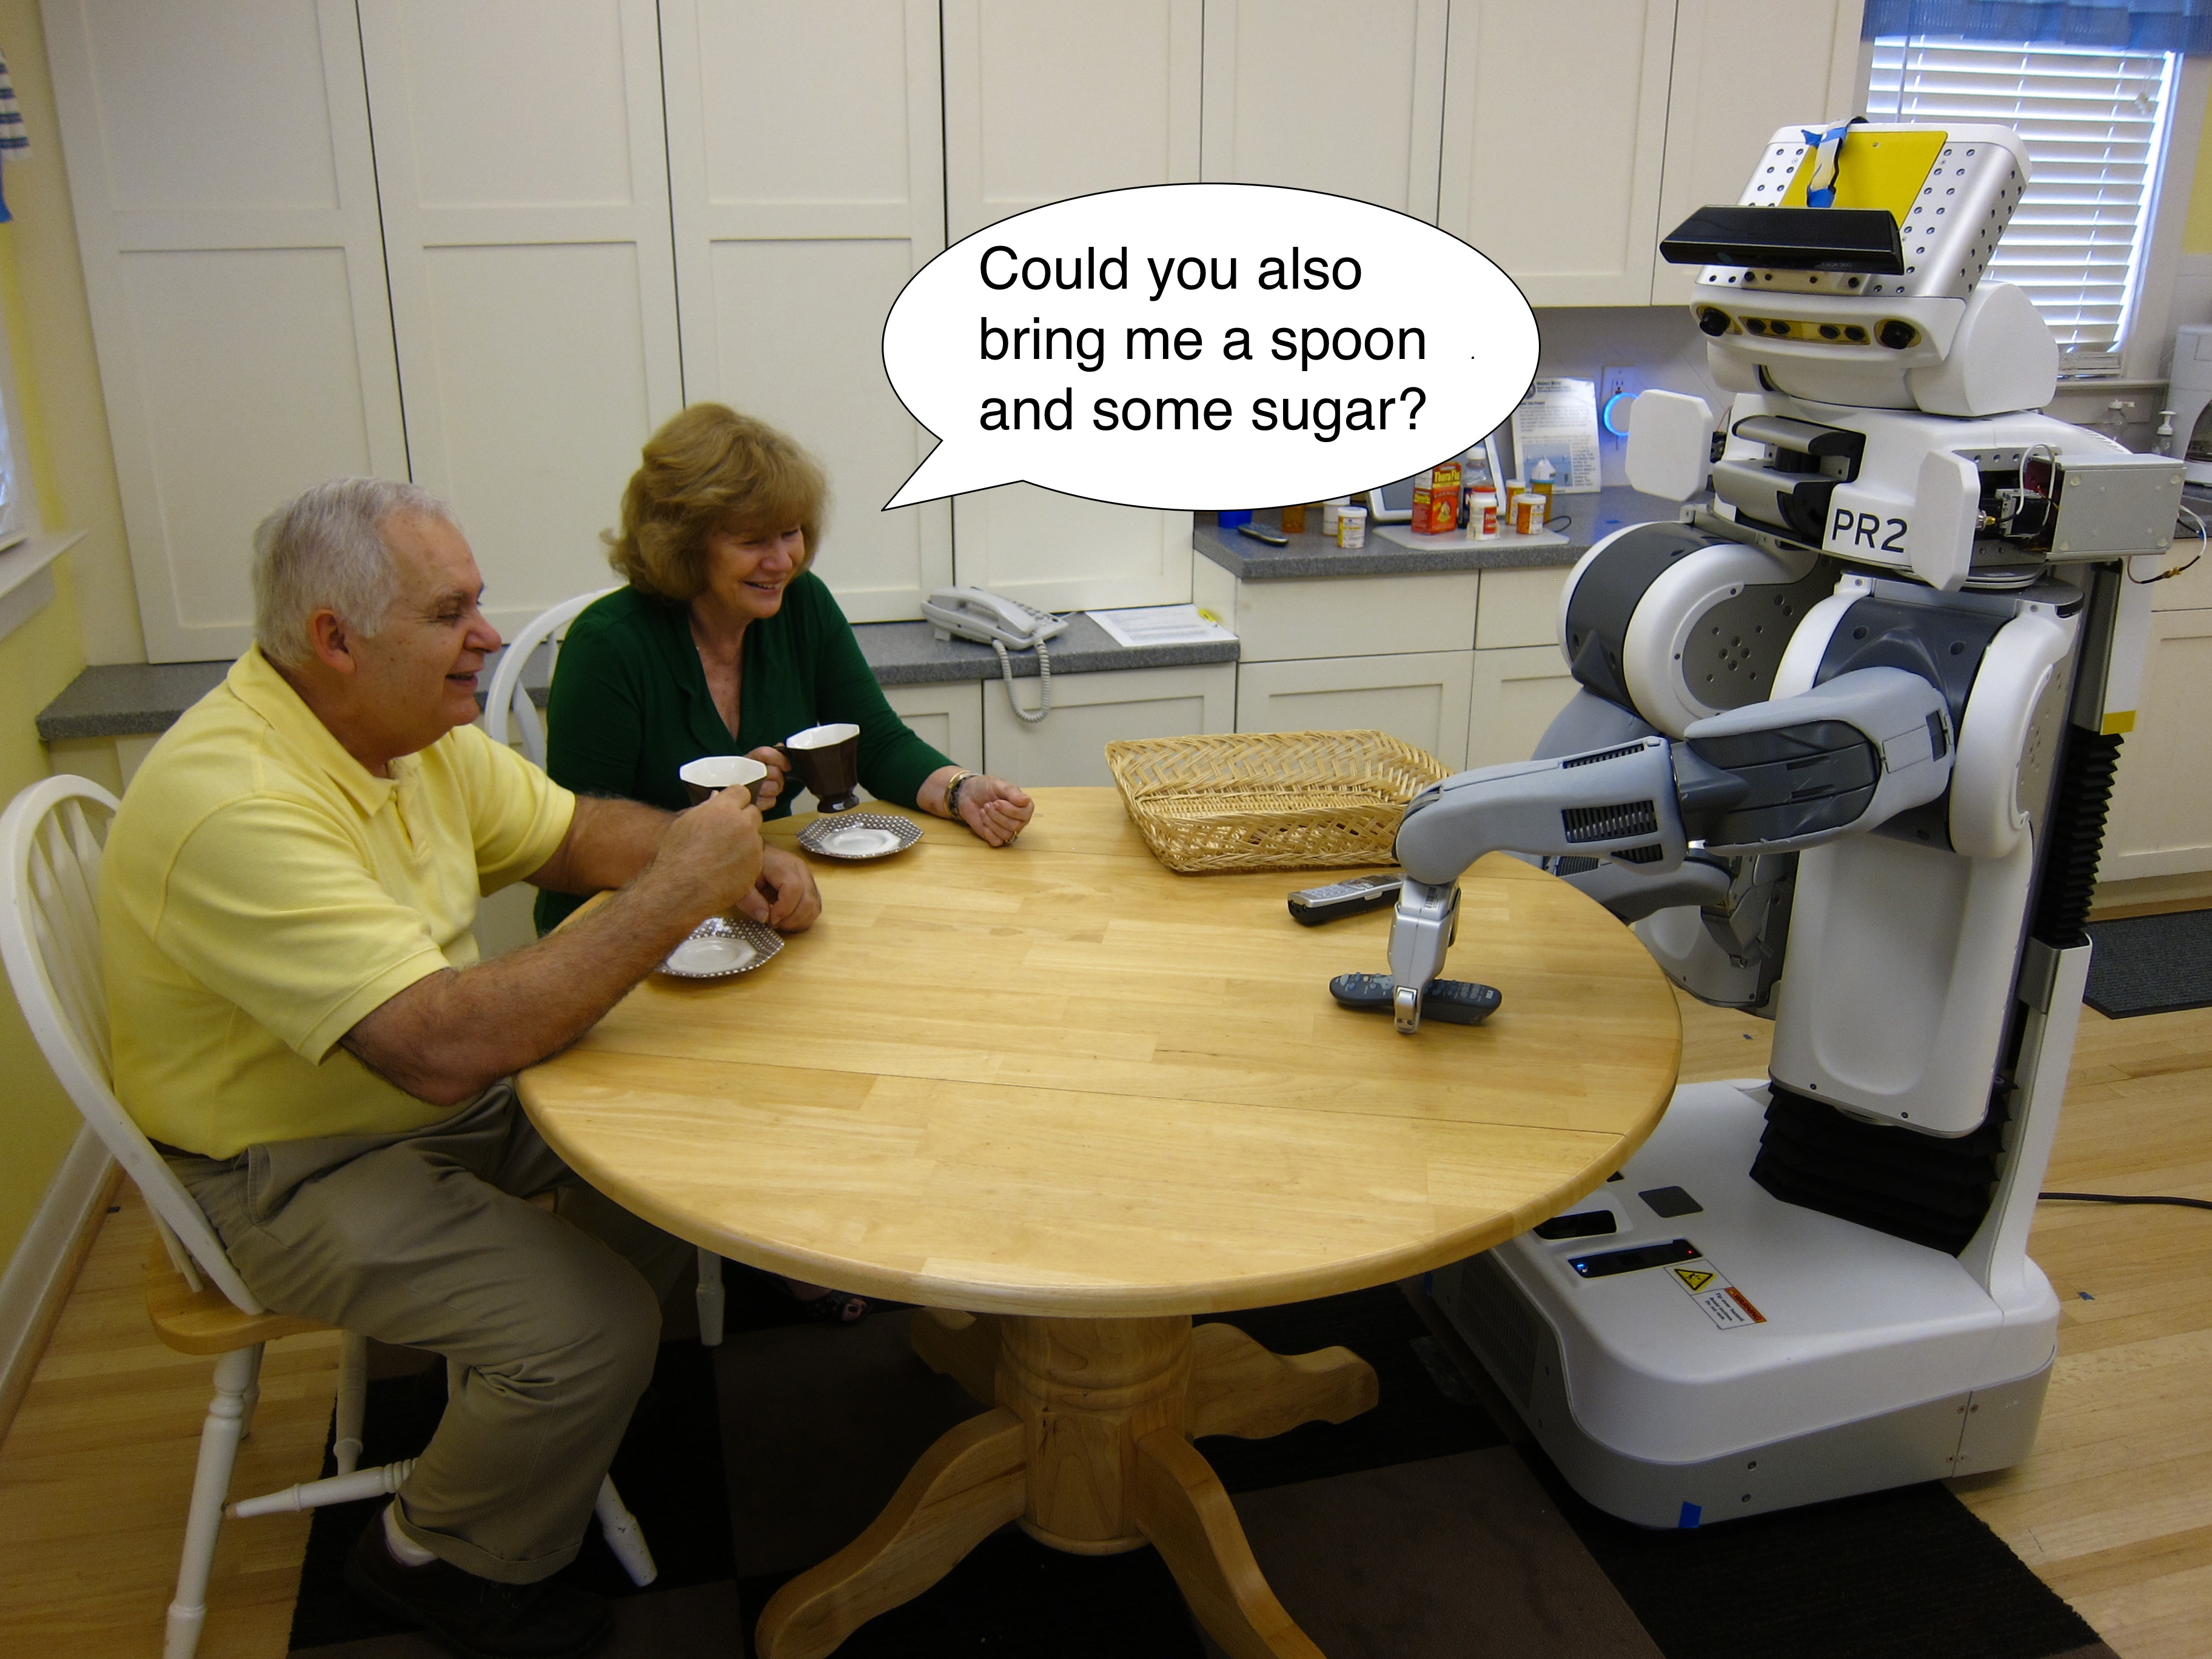
\includegraphics[width=3.2in]{img/robot_in_kitchen.jpg}

    \tiny{Original image courtesy of Wendy Rogers/Georgia Tech.}
  \end{center}
\end{frame}

\begin{frame}
  \frametitle{State of research}
\end{frame}

\begin{frame}
  \frametitle{Assumptions for the following treatment}
  \begin{itemize}
  \item There are no errors in the visual identification and classification of objects.
  \item The robot can successfully complete any movement and manipulation task,
    but motions take time, and are therefore expensive.
  \item The set of object types in the world is finite.
  \end{itemize}
\end{frame}

\begin{frame}
  \frametitle{Formulation of the problem}
  \begin{center}
    \vspace{-0.13in}
    Set of containers: $\{c_l\}$

    \spL[3-unknown-containers]

    Set of object types: $\{t_i\}$

    \spL[shape-universe-small]

    We want to find an object of type $q$ (the query type).

    \spL[blue-circle]

  \end{center}
\end{frame}

\begin{frame}
  \frametitle{Where is \spM[blue-circle]?}
  \begin{center}
    \spL[3-partially-observed-containers]

    \vspace{0.3in}

    Given that we have observed objects of types $\{t_{o_j}\}$ \\
    in container $c$, what is $\mathrm{P}(q \in c \, | \, \{t_{o_j}\})$ ?
  \end{center}
\end{frame}



\section{Generative Model of Container Contents}
\subsection{Co-occurrences}
\begin{frame}
  \frametitle{Composition of a container ($\theta$)}
  \begin{columns}
    \begin{column}{0.7\textwidth}
      \begin{center}
        \spM[shape-universe-small]\\
        \hspace{0.1in} 1 \hspace{0.2in} 2 \hspace{0.08in} 3 \hspace{0.08in} 4

        \begin{equation*}
          \theta' = (1, 2, 1, 3)
        \end{equation*}

        \begin{equation*}
          \theta = \frac{\theta'}{\norm{1}{\theta'}}
        \end{equation*}

        \begin{equation*}
          \theta = \Big ( \frac17, \frac27, \frac17, \frac37 \Big )
        \end{equation*}
      \end{center}
    \end{column}
    \begin{column}{0.3\textwidth}
      \spL[1-observed-container]
    \end{column}
  \end{columns}
\end{frame}


\begin{frame}
  \frametitle{Prior on Composition ($\theta$)}
  \begin{center}
    We need some prior probability distribution on $\theta$.
    \vspace{0.3in}

    A Dirichlet distribution is a common choice for this kind of application.
    However, the Dirichlet distribution doesn't have enough degrees of freedom to represent co-occurrences.
  \end{center}
\end{frame}

\begin{frame}
  \frametitle{Logistic Normal Prior on Composition ($\theta$)}
  \begin{center}
    \begin{equation*}
      \theta = ( \theta_1, \theta_2, \dots \theta_T )
    \end{equation*}

    \begin{equation*}
      \eta \sim \mathcal{N}(\mu, \Sigma)
    \end{equation*}

    $\sigma(\eta)$ transforms the normally distributed $\eta \in \mathbb{R}^T$ \\
    to $\theta \in \mathbb{R}_+^T$ such that $\norm{1}{\theta} = 1$.

    \begin{equation*}
      \theta_i = \sigma(\eta_i) = \frac{e^{\eta_i}}{\sum_{k=1}^{T}e^{\eta_k}}
    \end{equation*}
  \end{center}
\end{frame}

\begin{frame}
  \frametitle{Logistic Normal Prior on Composition ($\theta$)}
  \begin{center}
    Histogram of $\theta_i$
    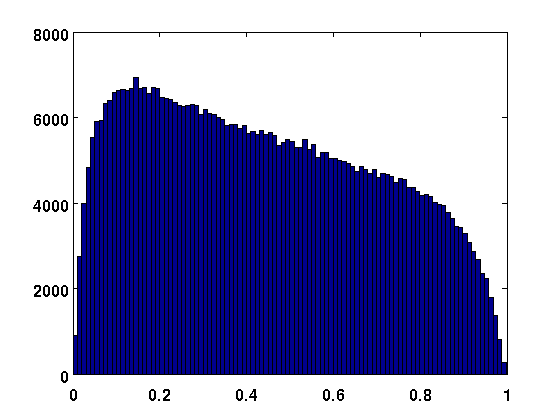
\includegraphics[scale=0.6]{img/log-normal-figs/hist-1.png}
  \end{center}
\end{frame}

\begin{frame}
  \frametitle{Logistic Normal Prior on Composition ($\theta$)}
  \begin{center}
    \vspace{-0.4in}
    \begin{equation*}
      \eta \sim \mathcal{N}(\mu, \Sigma)
    \end{equation*}
    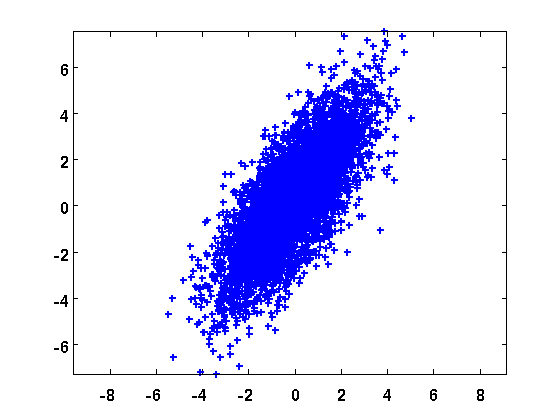
\includegraphics[scale=0.6]{img/log-normal-figs/normal-1.png}
  \end{center}
\end{frame}

\begin{frame}
  \frametitle{Logistic Normal Prior on Composition ($\theta$)}
  \begin{center}
    Histogram of $\theta_i$
    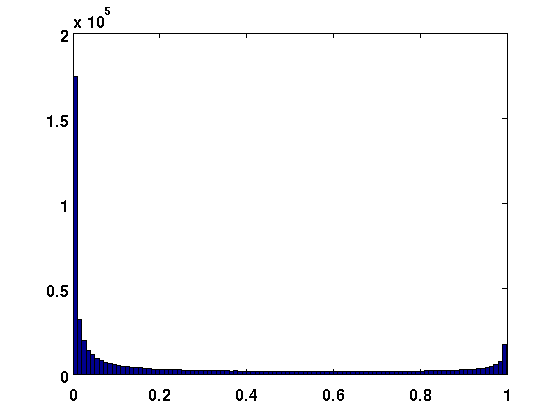
\includegraphics[scale=0.6]{img/log-normal-figs/hist-2.png}
  \end{center}
\end{frame}

\begin{frame}
  \frametitle{Logistic Normal Prior on Composition ($\theta$)}
  \begin{center}
    \vspace{-0.4in}
    \begin{equation*}
      \eta \sim \mathcal{N}(\mu, \Sigma)
    \end{equation*}
    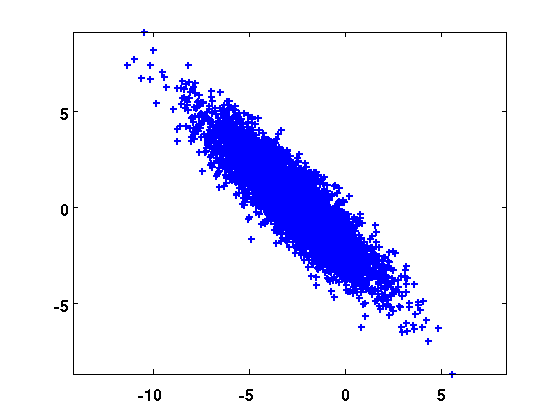
\includegraphics[scale=0.6]{img/log-normal-figs/normal-2.png}
  \end{center}
\end{frame}

%\begin{frame}
%  \frametitle{Inverse of Logistic Transformation}
%  \begin{center}
%    \begin{equation*}
%      \eta \sim \mathcal{N}(\mu, \Sigma)
%    \end{equation*}
%
%    \begin{equation*}
%      \theta_i = \sigma(\eta_i) = \frac{e^{\eta_i}}{\sum_{k=1}^{T}e^{\eta_k}}
%    \end{equation*}
%
%    \begin{equation*}
%      \eta_i = \sigma^{-1}(\theta_i)
%    \end{equation*}
%
%    \begin{equation*}
%      \eta_i \propto \ln \theta_i
%    \end{equation*}
%
%    WTF! THIS DOESN'T SEEM TO WORK! \\
%    HELP ME PROFESSOR WILLIAMS! YOU'RE MY ONLY HOPE!
%  \end{center}
%\end{frame}


\begin{frame}
  \frametitle{Likelihood Function}
  \begin{center}
    \vspace{-2em}
    \begin{align*}
    P(t_i | \eta) &= P(t_i | \theta) \\ 
    &\\
    &= \theta_i \\ 
    &\\
    & = \frac{e^{\eta_i}}{\sum_{k=1}^{T}e^{\eta_k}}
  \end{align*}

  \end{center}
\end{frame}

\begin{frame}
  \frametitle{Bayesian update}
  \begin{center}
    \begin{align*}
      P(\eta | t_i) &\propto P(t_i | \eta) P(\eta)\\
      &\\
      &=\frac{e^{\eta_i}}{\sum_{k=1}^{T}e^{\eta_k}} \mathcal{N}(\eta ; \mu, \Sigma)
    \end{align*}
  \end{center}
\end{frame}

\subsection{Spatial constraints}
\begin{frame}
  \frametitle{Packing a container}
  \begin{columns}
    \begin{column}{0.7\textwidth}
      \begin{center}
        \vspace{-3em}

        \begin{align*}
          &\begin{aligned}
            \theta\_samples = [ & \left( 0.4, 0.2, 0.1, 0.3 \right), \\
            & \left( 0.2, 0.1, 0.3, 0.4 \right) ]
          \end{aligned} \\
          &\invisible<1,17>{i = \alt<1-8>{0}{\alert<9>1} \; \longrightarrow \; 
            \theta = \alt<1-8>{\left( 0.4, 0.2, 0.1, 0.3 \right)}
            {\alert<9>{\left( 0.2, 0.1, 0.3, 0.4 \right)}}}\\
          &count = \alt<1-7>{0}{\alert<8>{1}}, \; total = \temporal<8-16>{0}{\alert<8>1}{\alert<17>2}\\
        \end{align*}

      \item<2-6,10-15>{Shape sampled from $\theta$: \phantom{\hspace{5em}}}\\
      \overlayL{green-rectangle}{2}
      \overlayL{red-square}{3}
      \overlayL{blue-circle}{4}
      \overlayL{red-square}{5}
      \overlayL{green-rectangle}{6}
      \overlayL{red-square}{10}
      \overlayL{green-rectangle}{11}
      \overlayL{orange-triangle}{12}
      \overlayL{orange-triangle}{13}
      \overlayL{red-square}{14}
      \overlayL{orange-triangle}{15}

      \item<17>$\mathbb{P}(q \in c_l|\{t_{o_j}\}) = \frac12$

      \end{center}
    \end{column}
    \begin{column}{0.3\textwidth}
      \overlayL{container-packing-1-1}{1-2}
      \overlayL{container-packing-1-2}{3}
      \overlayL{container-packing-1-3}{4}
      \overlayL{container-packing-1-4}{5}
      \overlayL{container-packing-1-5}{6}
      \overlayL{container-packing-1-6}{7-8}
      \overlayL{container-packing-2-1}{9-10}
      \overlayL{container-packing-2-2}{11}
      \overlayL{container-packing-2-3}{12}
      \overlayL{container-packing-2-4}{13}
      \overlayL{container-packing-2-5}{14}
      \overlayL{container-packing-2-6}{15}
      \overlayL{container-packing-2-7}{16-17}
    \end{column}
  \end{columns}
\end{frame}


\section{Search planning}
\begin{frame}
  \frametitle{Search planning}
  A robot searching for an object $q$ next removes an occluding object
  from the maximum likelihood container:

  \[\argmax_l{\mathbb{P}(q \in c_l|\{t_{o_j}\})}\]
\end{frame}

\begin{frame}
  \frametitle{Search}
  \begin{center}
    \overlayM{search-1}{1}
    \overlayM{search-2a}{2}
    \overlayM{search-2b}{3}
    \overlayM{search-3a}{4}
    \overlayM{search-3b}{5}
    \overlayM{search-4a}{6}
  \end{center}
\end{frame}

\section{Results}
\begin{frame}
  \frametitle{Algorithm speed}
\end{frame}

\section{Applications}
\begin{frame}
  \frametitle{Applications of the algorithm presented}
  \begin{columns}
    \begin{column}{0.5\textwidth}
    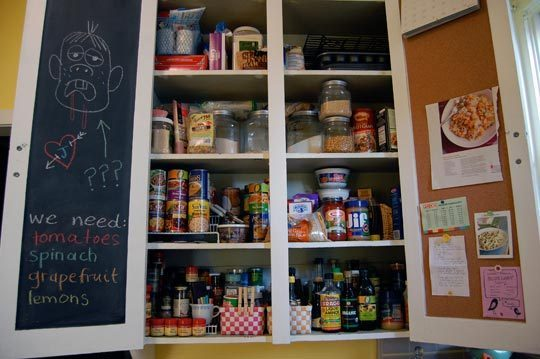
\includegraphics[width=\textwidth]{img/cupboard.jpg}

    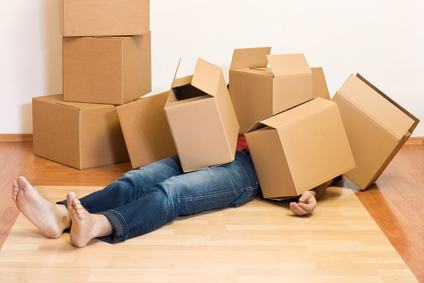
\includegraphics[width=\textwidth]{img/boxes.jpg}
    \end{column}
    \begin{column}{0.5\textwidth}
    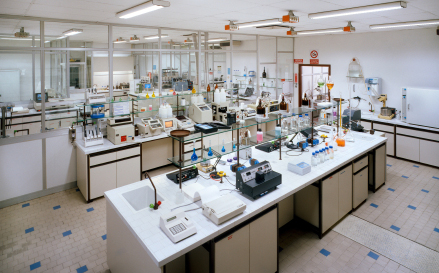
\includegraphics[width=\textwidth]{img/laboratory.jpg}

    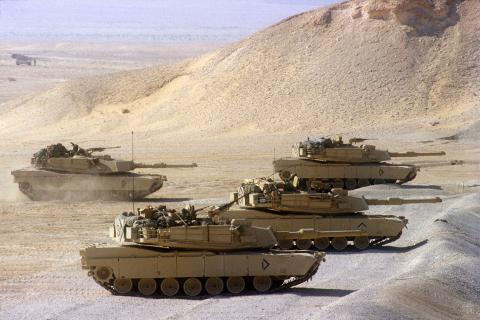
\includegraphics[width=\textwidth]{img/tanks.jpg}
    \end{column}
  \end{columns}
\end{frame}

\begin{frame}
  \frametitle{Applications of the general techniques learned}
  \begin{itemize}
    \item The Bayesian update is the same fundamental process as SLAM
  \end{itemize}
\end{frame}


\section{Conclusion}
\begin{frame}
\frametitle{Manipulation-based search for occluded objects}
\end{frame}

\begin{frame}
  \frametitle{Techniques (we hope) you've learned}
\end{frame}



\end{document}
